%%%%%%%%%%%%%%%%%%%%%%%%%%%%%%%%%%%%%%%%%%%%%%%%%%%%%%%%%%%%%%%%%%%%%%%%%%%%%%%
\section{Function approximation}\label{sec:mining}
%%%%%%%%%%%%%%%%%%%%%%%%%%%%%%%%%%%%%%%%%%%%%%%%%%%%%%%%%%%%%%%%%%%%%%%%%%%%%%%

The overall algorithm of function approximation is shown in figure~\ref{fig:approxAlg}
\begin{figure}[H]
\centering
\caption{Function approximation scheme}
\label{fig:approxAlg}
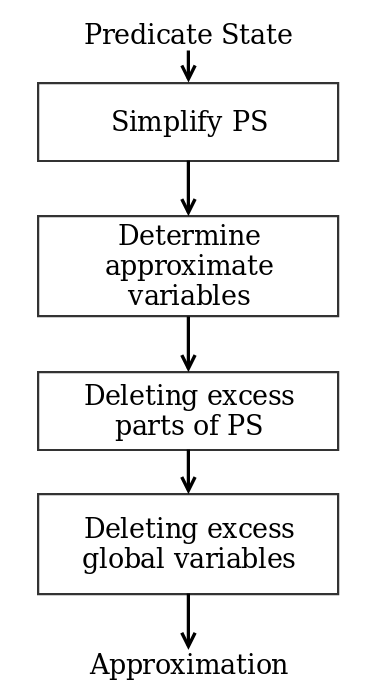
\includegraphics[keepaspectratio, width=\linewidth, height=8cm]{approxAlg}
\end{figure}


\subsection{Predicate State simplify}
At the beginning we must simplify predicate state, because LLVM uses static single assignment form (SSA), what complicates approximation. There are 2 simplify rules:
\begin{itemize}
\item if right side of current predicate equal or contained in left side of previous predicate, then we replace right side of current predicate by right side of previous;
\item for path predicates always replace value in condition by what was previously assigned
\end{itemize} 
An example of PS simplifying is shown in figure~\ref{fig:simEx}


\subsection{Determine approximate variables}
After simplifying we must to decide over which variables we will be approximate. In this work we decide to approximate over variables, which lead return values to constants. These variables are in path predicates on one of the branches which assigned the return value to the constant. This is done using algorithm~\ref{alg:lol}.

\subsection{Deleting excess parts of PS}
After determining approximate variables we need to extract parts of predicate state, which have influence on approximate variables. For this, first we must to traverse direct acyclic graph~(DAG) of program until we meet path predicate, which chose on previous step. Next we perfome reverse traverse with saving all code pieces.

For that algorithm we developed a mechanism of DAG traverse, which can consider all predicate state and it's distinct parts in direct and reverse order. After extracting we must to simplify predicate state by deleting unused global variables and empty constructions.


In this work we focus on dataflow predicates, specifically, on predicates corresponding to conditional statements over function arguments. The premise is that, if a condition checks an argument before a function call, this condition may capture an interesting precondition of this function.

Simplistically, one can collect all relevant conditions by slicing the call site PS w.r.t. function arguments. However, as LLVM IR uses static single assignment form~(SSA), each argument may be mapped to several LLVM IR variables, which greatly complicates slicing~(because of the need to track possible dependencies between variables).

To sidestep this problem, we gain advantage of the boundness of the underlying program model used in~BMC. As PS is fully unrolled and is, essentially, a directed acyclic graph~(DAG) in SSA form, we can propagate the equalities between variables along the DAG, removing most of the temporary variables and placing the function arguments directly in conditionals. An example of this equality predicate substitution is shown in figure~\ref{fig:equality-mapper-example}.

\begin{figure}[tbh]
\centering
\caption{Equality predicate substitution}
\label{fig:equality-mapper-example}
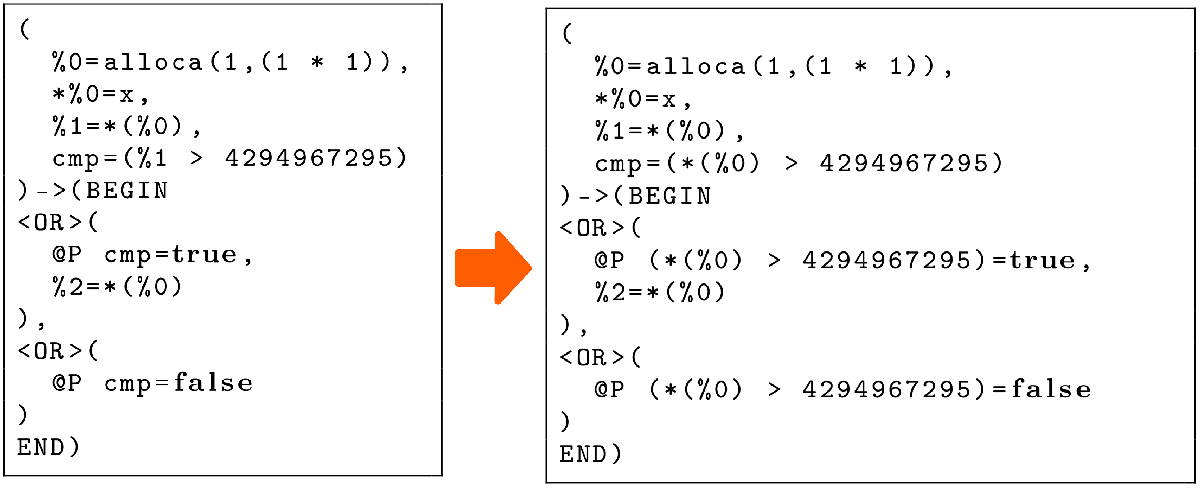
\includegraphics[width=\linewidth]{equality-mapper-example}
\end{figure}

After slicing the substituted PS, we get a DAG containing all conditionals interesting w.r.t. some function call. Before saving these predicates for subsequent summarization, there is one additional step needed. Some conditionals in alternative DAG branches might form a complete group over the possible arguments, which does not contribute to the interesting preconditions and should be removed.

This is done using algorithm~\ref{alg:complete-group-compaction}. We traverse the PS and remove all substates whose conditionals form a complete group. The check for a complete group is implemented using SMT solver as follows.

A set of conditionals~$C = \{c_1, c_2, \ldots, c_n\}$ form a complete group, if for every possible argument value at least one of $c_i$ is true. Therefore, if $\overline{ c_1 \lor c_2 \lor \ldots c_n }$ is unsatisfiable, these conditionals form a complete group; otherwise, there is at least one argument value which falsifies all conditionals, and they should be retained.

\begin{algorithm}[tbh]
\caption{PS compaction over complete conditionals}
\label{alg:complete-group-compaction}

\textbf{Input:}  $S$  --- sliced PS\\
\textbf{Output:} $S'$ --- compacted PS

\begin{algorithmic}
\State $S' \leftarrow empty$
\ForAll {$s \in S$}
    \State $c \leftarrow sliceConditions(s)$
    \If {$\neg isCompleteGroup(c)$}
        \State $S' \leftarrow S' + s$
    \EndIf
\EndFor
\end{algorithmic}
\end{algorithm}

The result of predicate mining is a set of compacted PS for every function call encountered during mining. These sets are stored in an external database%
\footnote{PS storage details are left outside the scope of this paper},
which is used to provide the aggregated information about interesting predicates over both the current and the previously analyzed programs.
